\documentclass[aspectratio=54,xcolor=dvipsnames]{beamer}
\usetheme{SimpleDarkBlue}

% Packages
\usepackage[utf8]{inputenc}
\usepackage{amsmath, amssymb}
\usepackage{graphicx}
\usepackage{hyperref}
\usepackage{physics}
\usepackage{dsfont}
\usepackage{verbatim}
\usepackage{listings}
\usepackage{booktabs}

\lstset{
    language=Octave,
    basicstyle=\ttfamily\tiny,
    numbers=left,
    numberstyle=\tiny\color{gray},
    stepnumber=1,
    numbersep=8pt,
    backgroundcolor=\color{gray!10},
    showspaces=false,
    showstringspaces=false,
    showtabs=false,
    frame=single,
    rulecolor=\color{gray!70},
    keywordstyle=\color{NavyBlue}\bfseries,
    commentstyle=\color{OliveGreen}\itshape,
    stringstyle=\color{BrickRed},
    breaklines=true,
    breakatwhitespace=true,
    tabsize=4,
    captionpos=b
}


% Title Information
\title{Computational Electromagnetics Project}
\subtitle{A One-Step Finite Element Method for Multiconductor Skin Effect Problems}
\author{Francesco Fischetti}
\institute{Politecnico di Milano}
\date{\today}

\begin{document}

% Title Slide
\begin{frame}
    \titlepage
\end{frame}

% Outline Slide
\begin{frame}{Outline}
    \tableofcontents
\end{frame}


\section{Recall: Maxwell's Equations}
\begin{frame}{Recall: Maxwell's Equations}
    Maxwell's equations in differential form are given by:
    \begin{align*}
        \nabla \cdot \vec{D} &= \rho \\
        \nabla \cdot \vec{B} &= 0 \\
        \nabla \times \vec{E} &= -\frac{\partial \vec{B}}{\partial t} \\
        \nabla \times \vec{H} &= \vec{J} + \frac{\partial \vec{D}}{\partial t}
    \end{align*}

    \begin{center}
    %\scriptsize
    \begin{tabular}{|c|l|c|}
        \hline
        Symbol & Quantity & Unit \\
        \hline
        $\vec{D}(\vec{r})$ & Electric flux density & $C/m^2$ \\
        $\vec{B}(\vec{r})$ & Magnetic flux density & $T$ \\
        $\vec{E}(\vec{r})$ & Electric field & $V/m$ \\
        $\vec{H}(\vec{r})$ & Magnetic field & $A/m$ \\
        $\vec{J}(\vec{r})$ & Current density & $A/m^2$ \\
        $\rho(\vec{r})$ & Volume charge density & $C/m^3$ \\
        \hline
    \end{tabular}
    %\normalsize
    \end{center}
\end{frame}

\begin{frame}{Recall: Constitutive Relations}
    For a linear and isotropic medium the constitutive relations read
    \begin{align*}
        \vec{D} &= \epsilon \vec{E} \\
        \vec{B} &= \mu \vec{H} \\
        \vec{J} &= \sigma \vec{E}
    \end{align*}
    \vspace{0.5em}
    where
    \begin{center}
    \begin{tabular}{|c|l|c|}
        \hline
        Symbol & Quantity & Unit \\
        \hline
        $\epsilon$ & Dielectric permittivity & $[F/m]$ \\
        $\mu$ & Magnetic permeability & $[H/m]$ \\
        $\sigma$ & Electric conductivity & $[S/m]$ \\
        \hline
    \end{tabular}
    \end{center}
\end{frame}

\section{Problem description and Electromagnetic Field Equations}
\begin{frame}{Problem description}
    Consider $\abs{C}$ infinitely long parallel conductors, with cross sections $\Omega_c$, with $c \in C$. Each conductor is assumed to have electrical conductivity $\sigma_c$, permittivity $\varepsilon_c$, and magnetic permeability $\mu_c$. The electromagnetic problem becomes two-dimensional with translational symmetry. We assume that the conductors are infinitely long in the $z$-direction.
        \begin{figure}[h]
            \centering
            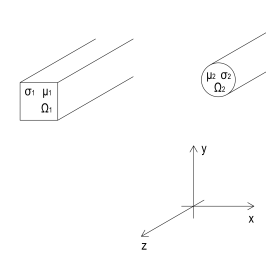
\includegraphics[width=0.35\textwidth]{Images/Conductors_figure.png}
            \caption{Geometry of the parallel conductors.}
            \label{fig:conductors}
        \end{figure}
\end{frame}

\begin{frame}{The Electromagnetic Field Equations I}
    In multipath eddy current problems where charges and displacement currents are negligible, the steady state time harmonic electromagnetic field is governed by:
    \begin{align}
        \nabla \cdot \tilde{\vec{D}} &= 0 \label{eq:divD} \\
        \nabla \cdot \tilde{\vec{B}} &= 0 \label{eq:divB} \\
        \nabla \times \tilde{\vec{E}} &= - j \omega \tilde{\vec{B}} \label{eq:curlE} \\
        \nabla \times \tilde{\vec{H}} &= \tilde{\vec{J}} \label{eq:curlH}
    \end{align}
    where $j$ is the imaginary unit and $\omega$ is the angular frequency. For the above complex fields, the time dependence is obtained by the substitution:
    \begin{equation*}
        \vec{V}(\vec{r}, t) = \sqrt{2} \cdot \Re \left\{ \tilde{\vec{V}}(\vec{r}) \cdot e^{j \omega t} \right\}
    \end{equation*}
    From now on, we will omit the tilde notation for the complex fields.
\end{frame}

\begin{frame}{The Electromagnetic Field Equations II}
    We introduce the Magnetic Vector Potential (MVP) as
    \begin{equation}
        \vec{B} = \mu \vec{H} = \nabla \times \vec{A}, \qquad \text{ with } \nabla \cdot \vec{A} = 0 \label{eq:divA}
    \end{equation}
    In this case all the variables are constant along $z$ (Figure~\ref{fig:conductors}), and:
    \begin{equation}
        \vec{H} = H_x \vec{e}_x + H_y \vec{e}_y, \qquad
        \vec{J} = J \vec{e}_z, \qquad
        \vec{A} = A \vec{e}_z. \label{ed:2D}
    \end{equation}
    Substituting \eqref{eq:divA} into the Maxwell's equations, we obtain that \eqref{eq:divB} is automatically satisfied, and \eqref{eq:curlH} becomes:
    \begin{equation}
        \nabla \times \left( \frac{1}{\mu} \nabla \times \vec{A} \right) = \vec{J}\label{eq:curlA}
    \end{equation}
    Using \eqref{ed:2D}, we can rewrite \eqref{eq:curlA} as:
    \begin{equation}
        \nabla \cdot \left( \frac{1}{\mu} \nabla A \right) = -J \label{eq:laplacianA}
    \end{equation}
\end{frame}

\begin{frame}{The Electromagnetic Field Equations III}
    The relationship between the electric field $\vec{E}$ and the magnetic vector potential $\vec{A}$ is obtained by substituting equation~\eqref{eq:divA} into equation~\eqref{eq:curlE} and integrating. The result is:
    \begin{equation}
        \vec{E} = -j\omega \vec{A} - \nabla \phi \label{eq:E}
    \end{equation}
    where $\phi$ is the electric scalar potential.
    \newline
    Define the source current density $\vec{J}_s$ and eddy current density $\vec{J}_e$ as:
    \begin{equation}
        \vec{J}_s = - \sigma \nabla \phi, \qquad
        \vec{J}_e = - j \omega \sigma \vec{A},  \qquad 
        \text{so that: } \vec{J} = \vec{J}_e + \vec{J}_s \label{eq:JsJe}
    \end{equation}
    Also define the source magnetic vector potential $\vec{A}_s$ as:
    \begin{equation}
        \vec{A}_s =  \frac{\vec{J}_s}{- j \omega \sigma}
    \end{equation}
    Writing equation~\eqref{eq:JsJe} in scalar form, we have: 
    \begin{equation}
        J = J_e + J_s = - j \omega \sigma A - \sigma \nabla \phi \cdot \vec{e}_z \label{eq:JsJe_scalar}
    \end{equation}
\end{frame}

\begin{frame}{The Electromagnetic Field Equations IV}
    \begin{block}{The System of Equations}
    Combining equations~\eqref{eq:laplacianA} and~\eqref{eq:JsJe_scalar}, we obtain the following system of equations:
    \begin{equation}\label{eq:system_equations}
        \left\{
        \begin{aligned}
            \nabla \cdot \left( \frac{1}{\mu} \nabla A \right) - j\omega \sigma A - j\omega \sigma A_s &= 0 
            \\[1em]
            - j\omega \sigma A - j\omega \sigma A_s &= J 
        \end{aligned}
        \right.
    \end{equation}
    \end{block}
    The system of equations must be solved subject to appropriate boundary conditions. In these equations, $A$ and $A_s$ are the unknowns, while $J$ is specified in the integral form:
    \begin{equation}
        \int_{\Omega_c} J \, ds = I_c
        \label{eq:current_constraint}
    \end{equation}
    where $I_c$ is the current flowing in conductor $c$ of cross-section $\Omega_c$, for $c \in C$.
\end{frame}

\begin{frame}{The Electromagnetic Field Equations: Remarks}
    \small
    \begin{itemize}[]
        \item $J_s$ is the external imposed current density by voltage source, it is a constant for each conductor. Also $A_s = \frac{J_s}{- j \omega \sigma}$ is a constant.
        \item $J_e = J_e(x,y)$ is the induced current density, it is a function of the magnetic vector potential $A(x,y)$.
        \item $\sigma$ is different from zero only in the conductors.  
    \end{itemize}
    The system of equations~\eqref{eq:system_equations} can be rewritten:
    \begin{subequations}
    \begin{equation*}
        \nabla \cdot \left( \frac{1}{\mu_0} \nabla A(x,y) \right)  = 0 \quad \quad \text{in } \Omega \setminus \bigcup_{c \in C} \Omega_c
    \end{equation*}
    \begin{equation*}
        \left\{
        \begin{aligned}
        \nabla \cdot \left( \frac{1}{\mu_0\mu_{r,c}} \nabla A(x,y) \right) - j\omega \sigma_c A(x,y) - j\omega \sigma_c A_{s,c} &= 0 
        \\[1em]
        - j\omega \sigma_c A(x,y) - j\omega \sigma_c A_{s,c} &= J_c 
        \end{aligned}
        \right.
        \qquad             
        \begin{array}{l}
            \text{in } \Omega_c \\
            \forall c \in C
        \end{array}
    \end{equation*}
    \end{subequations}

\end{frame}

\section{FEM Formulation}
\begin{frame}{Weak Formulation}
    \begin{footnotesize}
    Let $\mu$ and $\sigma$ be a piecewise constant functions defined as:
    \[
    \mu(\vec{r}) = 
    \begin{cases}
        \mu_0, & \vec{r} \in \Omega \setminus \bigcup_{c \in C} \Omega_c \\
        \mu_0\mu_{r,c} & \vec{r} \in \Omega_c, \, c \in C
    \end{cases}
    \qquad
    \sigma(\vec{r}) = 
    \begin{cases}
        0, & \vec{r} \in \Omega \setminus \bigcup_{c \in C} \Omega_c \\
        \sigma_c, & \vec{r} \in \Omega_c, \, c \in C
    \end{cases}
    \]
    And let $\mathds{1}_{\Omega_c}$ be the indicator function of the domain $\Omega_c$. \\
    \begin{block}{Weak Formulation}
    The weak formulation of~\eqref{eq:system_equations} reads: \\
    Find $A \in H^1_0(\Omega, \mathbb{C})$ and $A_{s,c} \in \mathbb{C}, \forall c \in C$ such that $\forall \phi \in H^1_0(\Omega)$:
    \begin{equation} 
        \int_{\Omega} \left( -\frac{1}{\mu} \nabla A \cdot \nabla \phi - j\omega \sigma A \, \phi - j\omega \left(\sum_{c \in C} \sigma_c A_{s,c} \mathds{1}_{\Omega_c} \right) \, \phi \right) ds = 0
        \label{eq:weak_formulation}
    \end{equation}
    Coupled with:
    \begin{equation}
        \int_{\Omega_c} \left(- j\omega \sigma_c A - j\omega \sigma_c A_{s,c} \right) ds = \int_{\Omega_c} J \, ds, \quad \forall c \in C
        \label{eq:current_constraint_weak}
    \end{equation}
    \end{block}
    Note that the weak formulation is applied only to the first equation of the system~\eqref{eq:system_equations}
    \end{footnotesize}
\end{frame}

\begin{frame}{Galerkin formulation I}
    Consider the finite element space $V_h \subset H^1(\Omega)$ spanned by the basis functions $\{\phi_i\}_{i=1}^{N}$, where $N$ is the number of nodes in the mesh. The approximate solution $A_h$ can be expressed as:
    \begin{align*}
        A_h = \sum_{i=1}^{N} A_i \phi_i
    \end{align*}
    Defining the matrices $S, M \in \mathbb{R}^{N \times N}$:
    \begin{align*}
        S_{ij} &= \int_{\Omega} \nabla \phi_i \cdot \nabla \phi_j \, ds, \\
        M_{ij} &= \int_{\Omega} \phi_i \phi_j \, ds, \\
    \end{align*}
    Defining the column vectors $\vec{q}_c \in \mathbb{R}^N, \, \forall c \in C $:
    \begin{align*}
        [\vec{q}_c]_i = \int_{\Omega} \mathds{1}_{\Omega_c} \phi_i \, ds = \int_{\Omega_c} \phi_i \, ds
    \end{align*}

\end{frame}

\begin{frame}{Galerkin formulation II}
    And defining the matrices $Q \in \mathbb{R}^{N \times \abs{C}}, W \in \mathbb{R}^{\abs{C} \times \abs{C}}$:
    \begin{align*}
        Q &= \left[
        \begin{array}{ccc}
            \vec{q}_1 & \ldots & \vec{q}_C
        \end{array}
        \right], \\
        W &= \left[
        \begin{array}{ccc}
            \abs{\Omega_1} & 0 & 0 \\
            0 & \ddots & 0 \\
            0 & 0 & \abs{\Omega_C}
        \end{array}
        \right]
    \end{align*}

    \begin{block}{Linear System of Equations}
    The equations~\eqref{eq:weak_formulation} and~\eqref{eq:current_constraint_weak} can be rewritten in matrix form as:
    \begin{equation}
        \left[
        \begin{array}{cc}
            \frac{1}{\mu} S + j\omega \sigma M & j\omega \sigma Q\\
            j\omega \sigma Q^t & j\omega \sigma W 
        \end{array}
        \right]
        \left[
        \begin{array}{c}
            \vec{A} \\
            \vec{A}_{s}
        \end{array}
        \right]
        =
        \left[
        \begin{array}{c}
            \vec{0} \\
            -\vec{I} 
        \end{array}
        \right]
    \end{equation}
    \end{block}
    Where $\vec{A} = [A_1, \ldots, A_N]^t$ and $\vec{A}_s = [A_{s,1}, \ldots, A_{s,C}]^t$ are the column vectors of unknowns, $\vec{I} = [I_1, \ldots, I_C]^t$ is the column vector of imposed currents, and $\mu$,$\sigma$ have the appropriate value depending on the position in the domain.
\end{frame}

\begin{frame}{FEM Formulation}
    \begin{block}{Finite Element Space}
    \[
    V_h = \left\{ v_h \in C^0(\overline{\Omega}) : v_h|_k \in \mathbb{P}^1(k)\ \forall k \in \mathcal{T}_h,\ v_h|_{\Gamma_D} = 0 \right\}
    \]
    where $\mathcal{T}_h$ is a triangulation of $\Omega$, $\mathbb{P}^1(k)$ denotes polynomials of degree 1 on element $k$, and $\Gamma_D$ is the Dirichlet boundary.
    \end{block}
    \begin{block}{Basis Functions}
    The basis functions $\{\phi_i^k(x, y)\}$ associated with each element $k$ are linear in $x$ and $y$:
    \[
    \phi_i^k(x, y) = a_i^k + b_i^k x + c_i^k y
    \]
    where the coefficients $a_i^k, b_i^k, c_i^k$ are determined such that
    \[
    \phi_i^k(x_j^k, y_j^k) = \delta_{ij}, \qquad \forall i, j = 1,2,3
    \]
    with $(x_j^k, y_j^k)$ the coordinates of the $j$-th node of element $k$.
    \end{block}
    
\end{frame}

\section{Implementation}
\subsection{Mesh Generation}
\begin{frame}{Implementation: mesh generation I}
    The mesh is generated using the \texttt{Gmsh} software. The mesh is defined in the file \texttt{two\_circ\_cond.geo}, which contains the geometry of the two conductors and the surrounding domain. The settable parameters for the mesh generation are:
    \begin{center}
         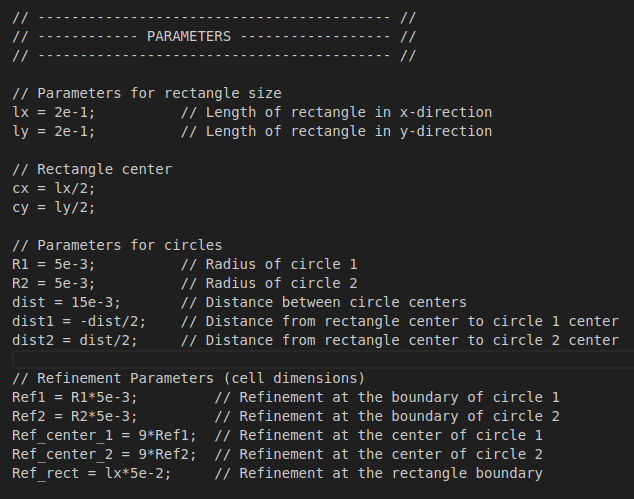
\includegraphics[width=0.7\textwidth]{Images/Gmsh_parameters.png}
    \end{center}
\end{frame}

\begin{frame}{Implementation: mesh generation II}
    The mesh sets different tags to the different regions of the domain, the tags are:
    \begin{center}
        \begin{tabular}{|c|l|}
            \hline
            Tag & Region \\
            \hline
            1 & Domain \\
            2 & Boundary of the domain \\
            11 & Conductor 1 \\
            12 & Conductor 2 \\
            \hline
        \end{tabular}
    \end{center}
    The mesh is then exported in \texttt{.m} format, a Matlab/Octave struct that contains all the mesh elements, saved in the file \texttt{mesh\_two\_circ\_cond.m}. This file is then read by the Octave code.
\end{frame}

\begin{frame}{Implementation: mesh generation III}
    \begin{center}
        \begin{minipage}{0.48\textwidth}
            \centering
            \begin{figure}
                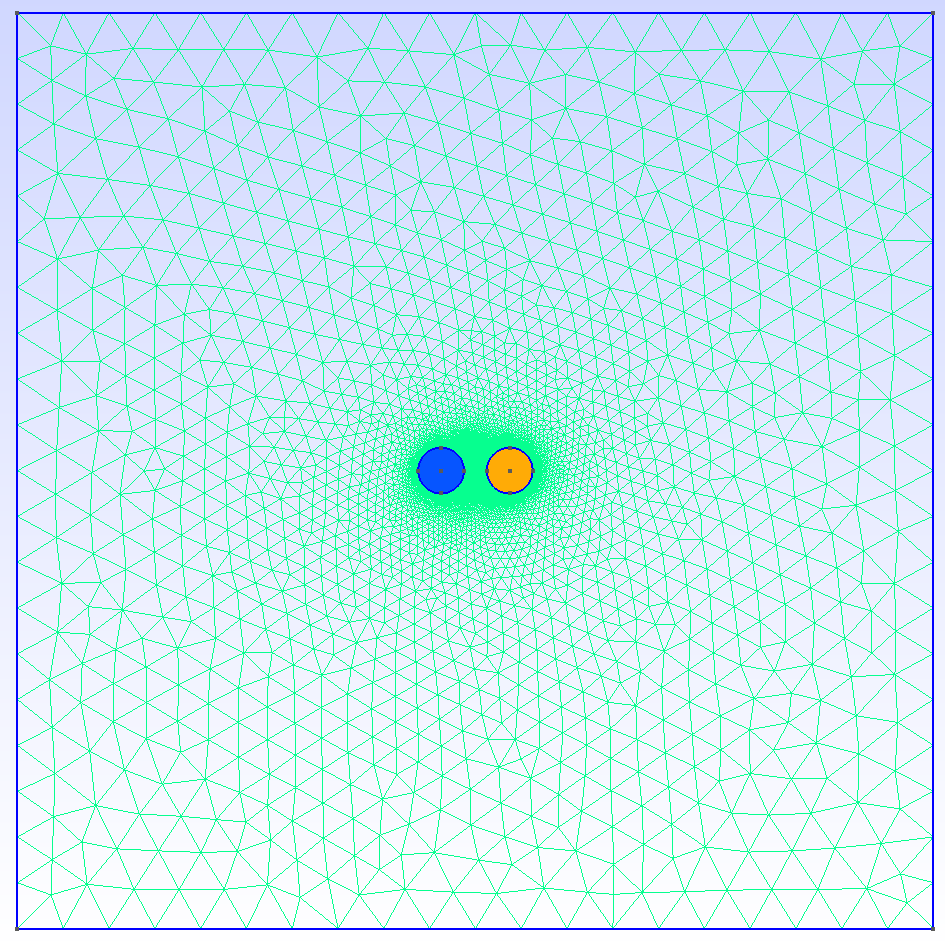
\includegraphics[width=\textwidth]{Images/Mesh_full.png}
                \caption{Full mesh of the domain.}
                \label{fig:mesh_full}
            \end{figure}
        \end{minipage}\hfill
        \begin{minipage}{0.48\textwidth}
            \centering
            \begin{figure}
                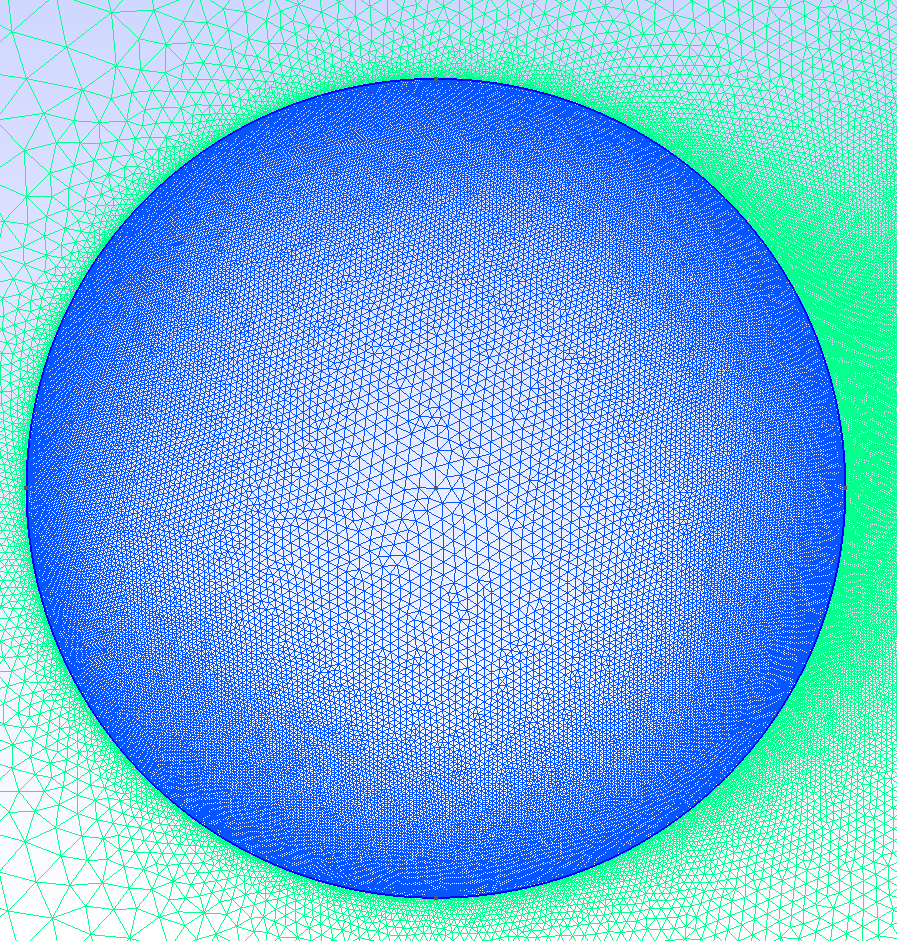
\includegraphics[width=\textwidth]{Images/Mesh_cond.png}
                \caption{Mesh around the conductors.}
                \label{fig:mesh_cond}
            \end{figure}
        \end{minipage}
    \end{center}
\end{frame}

\subsection{Main function}
\begin{frame}{Implementation: Main function (Description)}
    The function \texttt{FEM\_two\_conductors\_AC} implements the FEM method as described for 2 conductors. The main steps of the function are:
    \begin{enumerate}
        \item Load the necessary libraries (\texttt{msh}, \texttt{fpl}, \texttt{bim}).
        \item Load the mesh and saves the data to a struct (called \texttt{m}) and compute for each element area and gradient of basis functions.
        \item Extract the elements relative to the conductors and the boundary, compute $\mu$ and $\sigma$ with the correct element data.
        \item Assemble the Matrices $\frac{1}{\mu}S$, $j \omega \sigma M$, $j \omega \sigma Q$ and $j \omega \sigma W$, the full block system matrix and the block rhs vector.
        \item Solve the linear system applying homogeneous Dirichlet boundary conditions to obtain the total magnetic vector potential $A$ and the source magnetic vector potential $A_s$. Output the results in the specified format.
    \end{enumerate} 
\end{frame}

\begin{frame}[fragile]{1. FEM\_two\_conductors\_AC: Signature and Setup}
\small
\begin{lstlisting}
function [A, Js] = FEM_two_conductors_AC( mesh_file_name, freq, I_1, I_2, ...
                    mu_0, mu_r_1, mu_r_2, sigma_C_1, sigma_C_2, output_type)
  % Solve the eddy-current problem for two conductors at a given frequency.
  %
  % Inputs:
  %   mesh_file_name    : path to a .m mesh file generated by Gmsh
  %   freq              : excitation frequency [Hz]
  %   I_1, I_2          : total currents in conductors 1 and 2 [A]
  %   mu_0              : vacuum permeability [H/m]
  %   mu_r_1, mu_r_2    : relative permeabilities of conductors
  %   sigma_C_1, sigma_C_2 : conductivities of conductors [S/m]
  %   output_type       : can be "paraview" (results are written to .vtu files),
  %                       "octave" (results are plotted in Octave),
  %                       or "off" (no output is produced)
  %
  % Outputs:
  %   A               : nodal values of magnetic vector potential [T*m]
  %   Js              : source current density in each conductor [A/m^2]

  pkg load msh fpl bim

\end{lstlisting}
\end{frame}

\begin{frame}[fragile]{2. FEM\_two\_conductors\_AC: Mesh Loading \& Preprocessing}
\scriptsize
\begin{lstlisting}[firstnumber=22]
  ## MESH PARAMETERS
  %--- Define region identifiers in the Gmsh .m file
  cell_id.external = 1;     % outer domain tag
  cell_id.bc  = 2;          % outer boundary tag
  cell_id.conduct_1 = 11;   % first conductor tag
  cell_id.conduct_2 = 22;   % second conductor tag


  ## MESH LOADING
  disp('Loading data ...')
  source (mesh_file_name);

  %--- Build octave mesh structure 'm'
  m.p = msh.POS'([1 2], :); % mesh nodes coordinates as 2xN
  x = msh.POS(:, 1);        % x-coordinates
  y = msh.POS(:, 2);        % y-coordinates
  m.e = msh.LINES';         % mesh edges
  % (reformat Gmsh linedata to match bim format)
  m.e(5, :) = m.e(3, :); m.e(3, :) = 0; m.e(7, :) = 1;
  m.t = msh.TRIANGLES';     % mesh elements (mesh triangles)

  %--- compute area of each element (m.area), wheigh_i*det(Jacobian) in each 
  %    node of each element (m.wjacdet), and gradient of basis functions (m.shg)
  m = bim2c_mesh_properties (m);

  Nnodes = columns(m.p);  % Total number of nodes in the mesh
  Nelem = columns(m.t);   % Total number of elements in the mesh
  
\end{lstlisting}
\end{frame}

\begin{frame}[fragile]{3. FEM\_two\_conductors\_AC: Extracting Submeshes \& Element Data}
\scriptsize
\begin{lstlisting}[firstnumber=51]
  ## EXTRACT CONDUCTORS AND BOUNDARY CELLS AND NODES
  % conduct_1_nodes, conduct_2_nodes, bc_nodes contain respectively
  % the indices of the nodes in 1st conductor, 2nd conductor, external boundary.
  % While conduct_1_elem, conduct_2_elem contain respectively
  % the indices of the elements in 1st and 2nd conductor
  [~, conduct_1_nodes, conduct_1_elem] = msh2m_submesh(m, [], cell_id.conduct_1);
  [~, conduct_2_nodes, conduct_2_elem] = msh2m_submesh(m, [], cell_id.conduct_2);
  bc_nodes = bim2c_unknowns_on_side (m, cell_id.bc);


  ## SETTING PARAMETERS
  omega = 2*pi*freq;  % angular frequency, is a scalar

  %--- Build element mu vector: mu0 in external region, mu_0*mu_r in conductors
  mu = ones(Nelem, 1) * mu_0;
  mu(conduct_1_elem) = mu(conduct_1_elem) * mu_r_1;
  mu(conduct_2_elem) = mu(conduct_2_elem) * mu_r_2;

  %--- Build element indicator function for conductors
  ones_c_1 = zeros(Nelem, 1);
  ones_c_1(conduct_1_elem) = 1;
  ones_c_2 = zeros(Nelem, 1);
  ones_c_2(conduct_2_elem) = 1;

  %--- Build element sigma vector: 0 in external region, sigma_C in conductors
  sigma = sigma_C_1 * ones_c_1 + sigma_C_2 * ones_c_2;
  
\end{lstlisting}
\end{frame}

\begin{frame}[fragile]{4. FEM\_two\_conductors\_AC: Assembly of Linear System}
\scriptsize
\begin{lstlisting}[firstnumber=79]
  ## ASSEMBPLING SYSTEM
  disp('Assembling system ...')

  S = bim2a_laplacian(m, 1./mu, 1);           % Laplacian matrix with mu coeff

  M = reaction_full(m, omega.*sigma.*i, 1);   % Full mass matrix with coeff

  q_1 = bim2a_rhs(m, ones_c_1, 1);            % conductor 1 source vector

  q_2 = bim2a_rhs(m, ones_c_2, 1);            % conductor 2 source vector

  Q = [omega.*sigma_C_1.*i.*q_1, omega.*sigma_C_2.*i.*q_2]; % Q with coeff

  W = [omega*sigma_C_1*i*sum(q_1), 0; 0, omega*sigma_C_2*i*sum(q_2)]; % W
  % sum(q_1) and sum(q_2) are the areas of the conductors

  %--- Assemble global system
  System = [S+M, Q; Q.', W];
  Rhs = [zeros(Nnodes, 1); -I_1; -I_2];
  
\end{lstlisting}
\end{frame}

\begin{frame}[fragile]{5. FEM\_two\_conductors\_AC: Solve Linear System and Postprocessing}
\scriptsize
\begin{lstlisting}[firstnumber=100]
  ## SOLVE LINEAR SYSTEM
  disp('Solving system ...')

  % Internal nodes are all nodes except the boundary nodes, with the addition of
  % the two unknowns for the source magnetic vector potential in the conductors
  internal_nodes = setdiff (1:Nnodes + 2, bc_nodes);
  A_J = zeros(Nnodes + 2, 1);   % setup solution vector

  % solve linear system applying omogeneous Dirichlet boundary conditions
  A_J(internal_nodes) = System(internal_nodes, internal_nodes) \ Rhs(internal_nodes);

  ## GET RESULTS
  %--- Split solution into A (first N) and As (last 2)
  A = A_J(1:end-2);
  Js = [-omega * sigma_C_1 * i * A_J(end-1); -omega * sigma_C_2 * i * A_J(end)];

  %--- Compute current density J = -omega*sigma*i*A
  J = zeros(size(A));
  J(conduct_1_nodes) = -omega * sigma_C_1 * i * A(conduct_1_nodes) + Js(1);
  J(conduct_2_nodes) = -omega * sigma_C_2 * i * A(conduct_2_nodes) + Js(2);
  

  ## OUTPUT RESULTS
  if strcmp(output_type, "paraview") % Output results to paraview using fpl ...

\end{lstlisting}
\begin{lstlisting}[firstnumber=144]
  elseif strcmp(output_type, "octave")  % Plot results in octave using patch ...
\end{lstlisting}
\begin{lstlisting}[firstnumber=171]
endfunction
\end{lstlisting}
\end{frame}

\subsection{bim2c\_mesh\_properties}
\begin{frame}{bim2c\_mesh\_properties (Description)}
    The mesh properties (area, wheighted jacobian determinant (\texttt{wjacdet}), and shape functions gradients) are computed with the call to the function \texttt{bim2c\_mesh\_properties} of the \texttt{bim} package. This functions calls other subfunctions, one to compute the area (and \texttt{wjacdet}) of each element, and another to compute the gradients of the shape functions.
    The variables used in the subfunctions are:
    \begin{itemize}
        \item \texttt{p}: Matrix containing the coordinates of the mesh nodes (2xN).
        \item \texttt{e}: Matrix containing the edges of the boundary of the mesh (actually it is not used in this context)
        \item \texttt{t}: Matrix containing the elements of the mesh (4xNelem element connectivity + tags).
    \end{itemize}
    The results are saved in the mesh struct \texttt{m} under \texttt{m.area}, \texttt{m.wjacdet} and \texttt{m.shg}. The field \texttt{wjacdet} contains the weighted Jacobian determinants for each node in each element.
\end{frame}

\begin{frame}{bim2c\_mesh\_properties: Element Area I}
\small
Let each element have nodes with coordinates $((x_1,y_1), (x_2,y_2), (x_3,y_3))$.
\textbf{Jacobian matrix} for the affine map:
\[
    J \;=\;
    \begin{pmatrix}
        x_2 - x_1 & x_3 - x_1 \\[3pt]
        y_2 - y_1 & y_3 - y_1
    \end{pmatrix},
    \quad
    \det J \;=\;(x_2 - x_1)(y_3 - y_1)\;-\;(x_3 - x_1)(y_2 - y_1)
\]

\textbf{Element area}:
\[
    A_k \;=\;\tfrac12\,|\det J|
    \quad\Longrightarrow\quad
    A_k = \tfrac12\,\bigl|(x_2-x_1)(y_3-y_1)-(x_3-x_1)(y_2-y_1)\bigr|
\]
\textbf{In the code}:
\begin{itemize}
    \item weight: 1x3 node weights for reference triangle: $\mathtt{weight[i]} = \tfrac13$ 
    \item jacdet: 1 x Nelem Jacobian determinants for each element
    \item wjacdet: 3 x Nelem weighted Jacobian determinants for each node in each element: $\mathtt{wjacdet[i][k]} = \tfrac12 * \mathtt{weight[i]} * \mathtt{jacdet[k]}$ 
    \item area: Nelem x 1 element areas: $\mathtt{area[k]} = \sum_{i=1}^{3} \tfrac12 * \mathtt{weight[i]} * \mathtt{jacdet[k]}$
\end{itemize}
\end{frame}

\begin{frame}[fragile]{bim2c\_mesh\_properties: Element Area II}
\scriptsize
\begin{lstlisting}[firstnumber=374]
function [b] = computearea(p,e,t,string)

  % p: 2xN node coords, t: 4xNelem element connectivity + tags
  weight      = [1/3, 1/3, 1/3];    % equal weights for 3 nodes
  areakk      = 1/2;                % factor 1/2 in area formula
  Nelements   = columns(t);         % number of elements
  
  % Build Jacobian entries for each element K
  jac([1,2],:) = [ p(1,t(2,:)) - p(1,t(1,:)); p(1,t(3,:)) - p(1,t(1,:)) ];
  jac([3,4],:) = [ p(2,t(2,:)) - p(2,t(1,:)); p(2,t(3,:)) - p(2,t(1,:)) ];
  % determinant of Jacobian
  jacdet = jac(1,:) .* jac(4,:) - jac(2,:) .* jac(3,:);   
  
  % ... Error handling ...
\end{lstlisting}
\begin{lstlisting}[firstnumber=400]
  % Weighted jacobian for each local node i
  for inode = 1:3
    wjacdet(inode,:) = areakk .* jacdet .* weight(inode);
  endfor
  
  % Return weighted jacobian or area
  if string == "wjac"
    b = wjacdet;                  % 3 x Nelem array of 1/2*det*1/3
  elseif string == "area"
    b = sum(wjacdet)';            % Nelem x 1 vector of element areas
  endif

endfunction
\end{lstlisting}
\end{frame}

\begin{frame}{bim2c\_mesh\_properties: Gradient of shape functions I}
\small
Let each element have nodes with coordinates $((x_1,y_1), (x_2,y_2), (x_3,y_3))$.
\textbf{Gradient of linear “hat” basis} \(\varphi_i\) on each element:
\begin{align*}
    \nabla\varphi_1 = \frac{1}{det J_k}
        \begin{pmatrix} y_2 - y_3 \\[3pt] -(x_2 - x_3) \end{pmatrix},
    \\
    \nabla\varphi_2 = \frac{1}{det J_k}
        \begin{pmatrix} y_3 - y_1 \\[3pt] -(x_3 - x_1) \end{pmatrix},
    \\
    \nabla\varphi_3 = \frac{1}{det J_k}
        \begin{pmatrix} y_1 - y_2 \\[3pt] -(x_1 - x_2) \end{pmatrix}.
\end{align*}
Note that on each element the gradients are constant, and the determinant of the jacobian $det J_k$ is computed as before. \\
In code for each element 'k' these are assembled into a 2x3 array 'shg(:,:,k)'.
\end{frame}

\begin{frame}[fragile]{bim2c\_mesh\_properties: Gradient of shape functions II}
\scriptsize
\begin{lstlisting}[firstnumber=427]
function [shg] = shapegrad(p,t)
  
  ## Compute  the gradient of the hat functions
  
  x0 = p(1,t(1,:));
  y0 = p(2,t(1,:));
  x1 = p(1,t(2,:));
  y1 = p(2,t(2,:));
  x2 = p(1,t(3,:));
  y2 = p(2,t(3,:));

  denom = (-(x1.*y0) + x2.*y0 + x0.*y1 - x2.*y1 - x0.*y2 + x1.*y2);
  shg(1,1,:)  =  (y1 - y2)./denom;
  shg(2,1,:)  = -(x1 - x2)./denom;
  shg(1,2,:)  = -(y0 - y2)./denom;
  shg(2,2,:)  =  (x0 - x2)./denom;
  shg(1,3,:)  =  (y0 - y1)./denom;
  shg(2,3,:)  = -(x0 - x1)./denom;

endfunction
\end{lstlisting}
\end{frame}

\subsection{Matrices and RHS}
\begin{frame}[fragile]{Matrices and RHS: Assembly Algorithm}
\scriptsize
\begin{block}{Pseudocode Classic FEM}
\begin{verbatim}
for K = 1:Nelem
  for i = 1:3
    for j = 1:3
      I(i,j) = global node index of local node i in element K
      Compute local element matrix Mloc_K(i,j)
    endfor
  endfor
  Scatter into global matrix
endfor
\end{verbatim}
\end{block}

For performace reasons, in this code the assembly of all the matrices and RHS is done in a vectorized way, with the following structure:
\begin{block}{Pseudocode Octave Vectorized Assembly}
\begin{verbatim}
Mloc = zeros(3,3,Nelements);
for i = 1:3
  for j = 1:3
    Compute Mloc(i,j,:) in parallel over all elements
    Compute global node indices ginode(i,j,:), gjnode(i,j,:) 
  endfor
endfor
Single sparse call builds the global matrix
\end{verbatim}
\end{block}
\end{frame}

\begin{frame}{Laplacian matrix (Description)}
    The Laplacian matrix is computed in \texttt{bim2a\_laplacian}. \\
    Local assembly:
    \begin{align*}
        [L^{k}]_{ij} &= \int_{k} \epsilon \nabla \phi_i \cdot \nabla \phi_j \, ds = \epsilon_k \nabla \phi_{k,i} \cdot \nabla \phi_{k,j} \, Area_k
    \end{align*}
    \texttt{bim2a\_laplacian} has the following inputs:
    \begin{itemize}
        \item \texttt{mesh}: mesh struct.
        \item \texttt{epsilon}: vector of element data (1 x Nelem).
        \item \texttt{kappa}: vector of node data (1 x N).
    \end{itemize}

\end{frame}

\begin{frame}[fragile]{bim2a\_laplacian (Code)}
\scriptsize
\begin{lstlisting}[firstnumber=41]
function A = bim2a_laplacian (mesh, epsilon, kappa)
  % ... Check input ...
\end{lstlisting}
\begin{lstlisting}[firstnumber=51]
  p      = mesh.p;  % 2xN matrix of node coordinates
  t      = mesh.t;  % 4xNelem matrix of element connectivity + tags
  nnodes = columns(p); % number of nodes
  nelem  = columns(t); % number of elements
  % ... Turn scalar input to a vector of appropriate size ...
\end{lstlisting}
\begin{lstlisting}[firstnumber=69]
  Lloc = zeros(3, 3, nelem); % 3x3 matrix for each element in the mesh

  % Use inverse average to account for the node diffusion coefficient.
  % In this case, kappa is one, so the expression is equivalent to:
  % kappaepsilonareak = epsilon .* mesh.area;
  kappaepsilonareak = reshape (3./sum (1./kappa(:)(mesh.t (1:3)), 1)(:) .* epsilon(:) .* mesh.area(:), 1, 1, nelem);
  shg = mesh.shg(:,:,:);  % 2x3xNelem matrix of gradients of shape functions
  
  ## Computation
  for inode = 1:3
    for jnode = 1:3
      ginode(inode,jnode,:) = mesh.t(inode,:); % global node indices
      gjnode(inode,jnode,:) = mesh.t(jnode,:);
      Lloc(inode,jnode,:)   = sum (shg(:,inode,:) .* shg(:,jnode,:), 1) .* kappaepsilonareak;
    endfor
  endfor

  ## Assemble the local (full) matrices into one global (sparse) matrix
  A = sparse (ginode(:), gjnode(:), Lloc(:));
endfunction
\end{lstlisting}
\end{frame}

\begin{frame}{Mass matrix (Description)}
    The mass matrix is computed in \texttt{reaction\_full}. \\
    Local assembly:
    \begin{align*}
        [B^{k}]_{ij}
        = \int_{k} \delta_{k}\,\varphi_i\,\varphi_j \,dA
        = \delta_{k}\,det(J_k)\,\int_{\hat{k}} \hat{\varphi}_i\,\hat{\varphi}_j \,d\hat{A} = \\
        = \delta_{k}\,2\,\mathrm{Area}_{k}\,\frac{1}{24}
          \begin{pmatrix}2&1&1\\1&2&1\\1&1&2\end{pmatrix}_{ij}
    \end{align*}
    where $\hat{k}$ is the reference triangle and $\hat{\varphi}_i$ are the reference basis functions. \\
    \texttt{reaction\_full} has the following inputs:
    \begin{itemize}
        \item \texttt{mesh}: mesh struct.
        \item \texttt{delta}: vector of element data (1 x Nelem).
        \item \texttt{zeta}: vector of node data (1 x N).
    \end{itemize}
\end{frame}

\begin{frame}[fragile]{reaction\_full (Code)}
\scriptsize
\begin{lstlisting}[language=Octave,firstnumber=19]
function C = reaction_full(mesh, delta, zeta)
  % ... Check input ...
\end{lstlisting}
\begin{lstlisting}[firstnumber=29]
  p      = mesh.p;    % 2xN node coords
  t      = mesh.t;    % 4xNelem connectivity + tags
  nnodes = columns(p); % number of nodes
  nelem  = columns(t); % number of elements
  % ... Turn scalar input to a vector of appropriate size ...
\end{lstlisting}
\begin{lstlisting}[firstnumber=46]
  % Local element matrices: one 3x3 block per element
  Blocmat = zeros(3,3,nelem);

  % Use inverse average to account for the node coefficient.
  % In this case, zeta is one, so the expression is equivalent to:
  % zetadeltaareak = delta .* mesh.area;
  zetadeltaareak = reshape (3./sum (1./zeta(:)(mesh.t (1:3)), 1)(:) .* delta(:) .* mesh.area(:), 1, 1, nelem);
  phi_ij  = [2 1 1; 1 2 1; 1 1 2] / 24; % integrals of reference basis functions

  % Build each local block in vectorized loops
  for inode = 1:3
    for jnode = 1:3
      ginode(inode,jnode,:) = mesh.t(inode,:);   % global rows
      gjnode(inode,jnode,:) = mesh.t(jnode,:);   % global cols
      Blocmat(inode, jnode, :) = phi_ij(inode, jnode) .* 2 .* zetadeltaareak;
    endfor
  endfor

  ## Assemble the local (full) matrices into one global (sparse) matrix
  C = sparse (ginode(:), gjnode(:), Blocmat(:));
endfunction
\end{lstlisting}
\end{frame}

\begin{frame}{RHS vector (Description)}
    The load vector is computed in \texttt{bim2a\_rhs}. \\
    Local assembly on element \(k\):
    \[
      [b^{k}]_{i}
      = \int_{k} f_{k}\,g(x)\,\varphi_i(x)\,dA
      \;\approx\;
      f_{k}\,g(x_{i})\,\frac{\mathrm{Area}_{k}}{3}
      \;=\;
      f_{k}\,g_{i}^{k}\,\texttt{wjacdet}_{i,k}
    \]
    where \(\texttt{wjacdet}_{i,k}=\tfrac12\tfrac13\det(J_k)\).  
    \bigskip

    \texttt{bim2a\_rhs} has the following inputs:
    \begin{itemize}
      \item \texttt{mesh}: mesh struct, with \texttt{wjacdet} precomputed.
      \item \texttt{f}: element-wise source term (1 x Nelem).
      \item \texttt{g}: nodal coefficient (1 x N).
    \end{itemize}
\end{frame}

\begin{frame}[fragile]{bim2a\_rhs (Code)}
\scriptsize
\begin{lstlisting}[language=Octave,firstnumber=40]
function b = bim2a_rhs(mesh, f, g)
  % ... input checks ...
\end{lstlisting}
\begin{lstlisting}[firstnumber=50]
  nnodes = columns(mesh.p);
  nelem  = columns(mesh.t);
  % ... Turn scalar input to a vector of appropriate size ...
\end{lstlisting}
\begin{lstlisting}[firstnumber=68]
  % Extract g at each element's nodes
  g = g(mesh.t(1:3,:));        % 3xNelem matrix
  wjacdet = mesh.wjacdet;      % 3xNelem weighted jacobian

  % Build local contributions: Blocmat(i,K) = f_K * g_i^K * wjacdet(i,K)
  Blocmat = zeros(3, nelem);
  for inode = 1:3
    Blocmat(inode,:) = f.' .* g(inode,:) .* wjacdet(inode,:);
  endfor

  % Global node indices for each local position
  gnode = mesh.t(1:3,:);       % 3xNelem

  % Assemble sparse right-hand side vector
  b = sparse(gnode(:), 1, Blocmat(:));
endfunction
\end{lstlisting}
\end{frame}

\subsection{Running the simulations}
\begin{frame}[fragile]{Running the simulation}
To run the simulation and visualize the results, the small script \texttt{FEM\_eddy\_currents.m} can be used. 
\begin{lstlisting}[firstnumber=1]
clear

## PHYSICAL PARAMETERS

I_1 = 1;                % current in conductor 1 [A]
I_2 = -1;               % current in conductor 2 [A]
freq = 1e3;             % frequency [Hz]

sigma_C_1 = 58e6;       % conductivity of conductor 1 [S/m]
sigma_C_2 = sigma_C_1;  % conductivity of conductor 2 [S/m]

mu_0 = 4*pi*1e-7;       % vacuum permeability [H/m]
mu_r_1 = 1;             % permeability of conductor 1
mu_r_2 = 1;             % permeability of conductor 2

mesh_file_name = "mesh_two_circ_cond.m";

output_type = "paraview";  % The options are: "octave", "paraview", "off"
% For performance reasons (expecially with fine meshes) the option "paraview" is recommended if the software is available

[A, Js] = FEM_two_conductors_AC(mesh_file_name, freq, I_1, I_2, mu_0, mu_r_1, mu_r_2, sigma_C_1, sigma_C_2, output_type);
\end{lstlisting}
\end{frame}

\begin{frame}[fragile]{Impedance error}
\scriptsize
To compute the impedance error and plot in function of frequency, the script \texttt{FEM\_impedance\_two\_conductors.m} can be used. 
\begin{lstlisting}[firstnumber=1]
## SETTABLE PARAMETERS
sigma_C = 58e6;         % conductivity of both conductors [S/m]
mu_0 = 4*pi*1e-7;       % vacuum permeability [H/m]
mu_r_1 = 1;             % permeability of conductor 1
mu_r_2 = 1;             % permeability of conductor 2
freq_list = logspace(3, 6, 7);  % analyzed frequencies [Hz]
% Parameters that need to be consistent with the mesh 
mesh_file_name = "mesh_two_circ_cond.m";
radius = 5e-3;                % Radius of both conductors [m]
dist = 15e-3;                 % Distance between circle centers [m]
Ref_bound_C = radius*5e-3;    % Mesh refinement at the boundary of conductors [m]
Ref_center_C = 9*Ref_bound_C; % Mesh refinement at the center of conductors [m]

## COMPUTATIONS
I_1 = 1; I_2 = -1;
R_fem = zeros(size(freq_list)); L_fem = zeros(size(freq_list));
R_an = zeros(size(freq_list)); L_an = zeros(size(freq_list));
for n_f = 1:numel(freq_list)
  freq = freq_list(n_f);
  % Numerical solution
  [A, Js] = FEM_two_conductors_AC(mesh_file_name, freq, I_1, I_2, mu_0, mu_r_1, mu_r_2, sigma_C, sigma_C, "off");
  Z_self_1 = Js(1) / (sigma_C * I_1);
  R_fem(n_f) = real(Z_self_1);  % Numerical resistance
  L_fem(n_f) = imag(Z_self_1)/(2*pi*freq); % Numerical inductance
  % Analytical solution
  [R_an(n_f), L_an(n_f)]= analytical_two_circular_conductors (radius, dist, sigma_C, mu_r_1, mu_r_2, freq); % Analytical resistance and inductance
endfor
error_R = 100*(R_fem-R_an)./R_an; error_L = 100*(L_fem-L_an)./L_an;
% ... Plot the results in loglog scale ...
\end{lstlisting}
\end{frame}

\section{Results}
\begin{frame}{Simulation Results}
    The following results are obtained with the parameters:
    \begin{table}[H]
    \centering
    \begin{tabular}{l c r}
      \toprule
      \textbf{Parameter} & \textbf{Value} & \textbf{Units} \\
      \midrule
        Radius conductor 1   & $5 \times 10^{-3}$         & $m$      \\
        Radius conductor 2   & $5 \times 10^{-3}$         & $m$      \\
        Distance between centers  & $1.5 \times 10^{-2}$       & $m$         \\
        Mesh dimension at conductors boundary & $2.5 \times 10^{-5}$  &  $m$  \\
        Mesh dimension at conductors center & $2.25 \times 10^{-4}$  &  $m$  \\
        Imposed current in conductor 1 & $1$        & $A$      \\
        Imposed current in conductor 2 & $-1$       & $A$    \\
        Conductivity of conductor 1  & $58 \times 10^6$ & $S/m$    \\
        Conductivity of conductor 2  & $58 \times 10^6$ & $S/m$    \\
        Vacuum permeability & $4\pi\times10^{-7}$ & $H/m$    \\
        Relative permeability of conductor 1 & $1$ & - \\
        Relative permeability of conductor 2 & $1$ & - \\
      \bottomrule
    \end{tabular}
    \caption{Simulation parameters}\label{tab: Parameters}
    \end{table}
\end{frame}

\begin{frame}{Simulation Results: Magnetic Vector Potential}
    \scriptsize
    \begin{figure}[H]
        \centering
        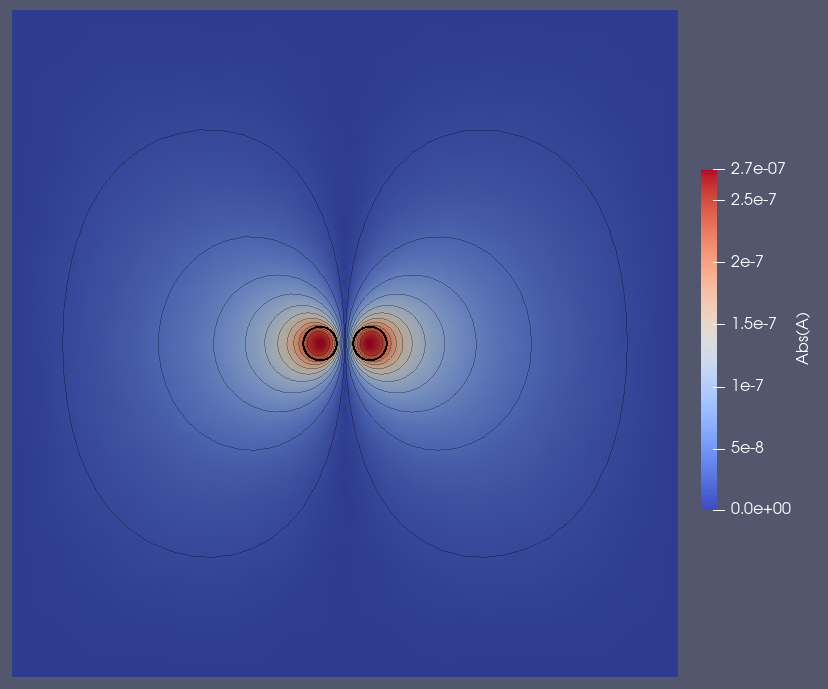
\includegraphics[width=0.75\textwidth]{Images/Abs_A_contour.png}
        \caption{Magnetic vector potential magnitude $[T \cdot m]$ at $f = 1 \times 10^3$ Hz. \newline In gray the contour lines, in black the boundary of the conductors.}
        \label{fig: A_1kHz}
    \end{figure}
\end{frame}

\begin{frame}{Simulation Results: Current Density}
    \scriptsize
    \begin{figure}[H]
        \centering
        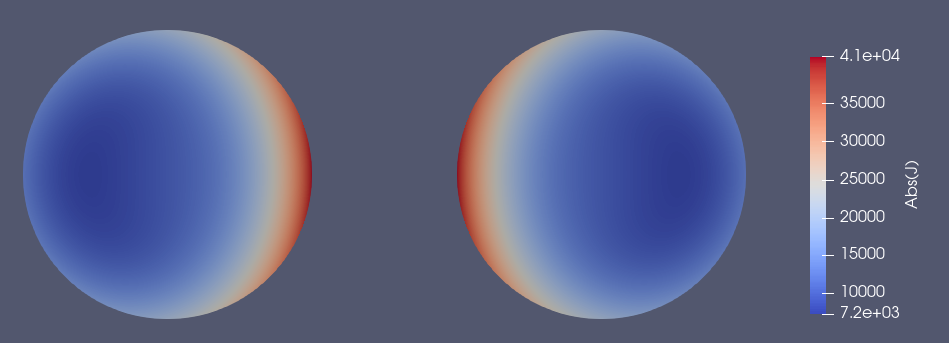
\includegraphics[width=0.9\textwidth]{Images/Abs_J.png}
        \caption{Current density magnitude $[A/m^2]$ at $f = 1 \times 10^3$ Hz inside the conductors.}
        \label{fig: J_1kHz}
    \end{figure}
\end{frame}

\begin{frame}{Simulation Results: Resistance and Inductance error}
    \scriptsize
    \begin{center}
    \begin{minipage}{0.49\textwidth}
        \centering
        \begin{figure}[H]
            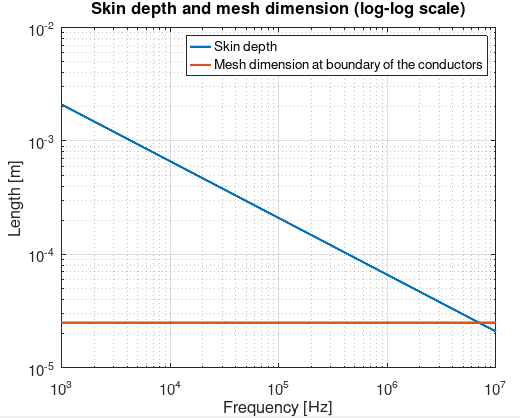
\includegraphics[width=\textwidth]{Images/Skin_depth.png}
            \caption{Skin depth $\delta$ [m] as a function of frequency $f$ [Hz]. The skin depth is defined as $\delta = \sqrt{\frac{2}{\omega \mu \sigma}}$, and it represents the depth at which the current density falls to $1/e$ of its value at the surface.}
        \end{figure}
    \end{minipage}\hfill
    \begin{minipage}{0.49\textwidth}
        \centering
        \begin{figure}[H]
            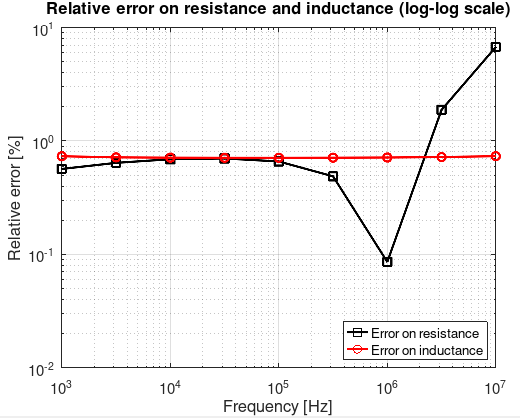
\includegraphics[width=\textwidth]{Images/Error_plot.png}
            \caption{Relative error in resistance and inductance as a function of frequency. The resistance error is defined as $\abs{100 \times \frac{R_{fem} - R_{an}}{R_{an}}}$, and the inductance error as $\abs{100 \times \frac{L_{fem} - L_{an}}{L_{an}}}$.}
        \end{figure}
    \end{minipage}
    \end{center}
\end{frame}

\begin{frame}{Simulation Results: Skin Depth visualization}
    \scriptsize
    \begin{center}
        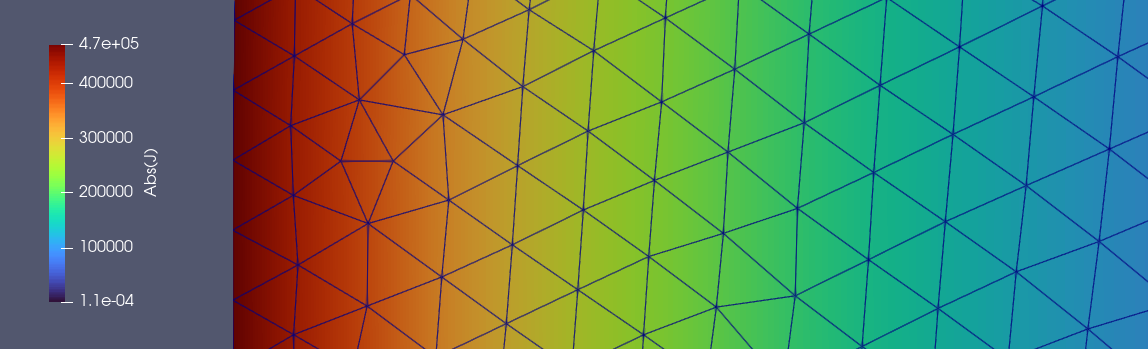
\includegraphics[width=0.6\textwidth]{Images/Skin_depth_f_1e5.png}\\
        \scriptsize $\abs{J}$ at $f = 1 \times 10^5$ Hz. $\delta = 2.09 \times 10^{-4}$ m, $h_k = 2.5 \times 10^{-5}$ m. 
        \vspace{0.5em}

        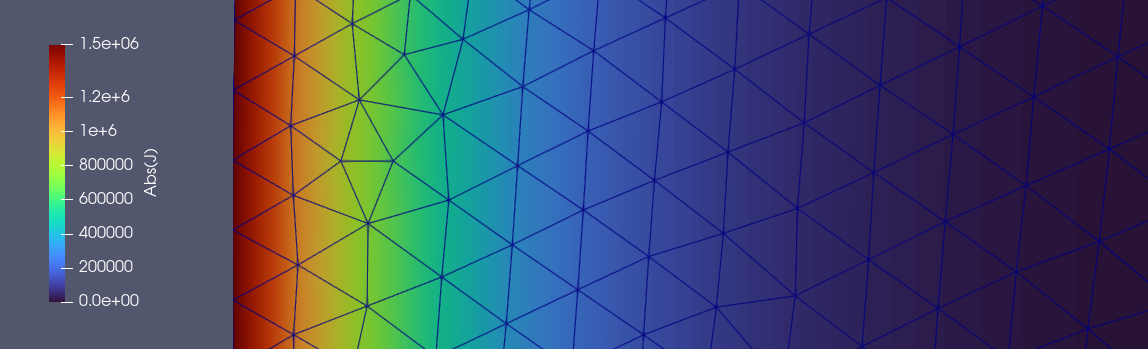
\includegraphics[width=0.6\textwidth]{Images/Skin_depth_f_1e6.png}\\
        \scriptsize $\abs{J}$ at $f = 1 \times 10^6$ Hz. $\delta = 6.61 \times 10^{-5}$ m, $h_k = 2.5 \times 10^{-5}$ m.
        \vspace{0.5em}

        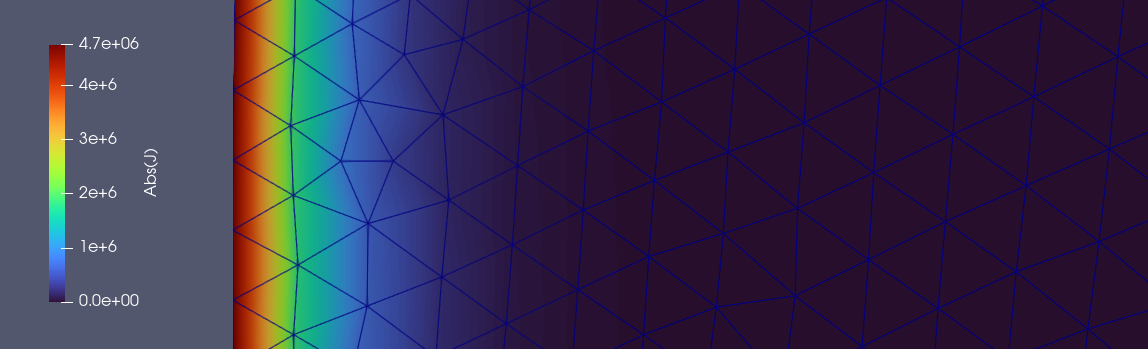
\includegraphics[width=0.6\textwidth]{Images/Skin_depth_f_1e7.png}\\
        \scriptsize $\abs{J}$ at $f = 1 \times 10^7$ Hz. $\delta = 2.09 \times 10^{-5}$ m, $h_k = 2.5 \times 10^{-5}$ m. \\ 
        In this case the mesh is not refined enough, error on resistance is about 10\%.
    \end{center}
\end{frame}

\begin{frame}{Simulation Results: BEM and FEM comparison}
    \scriptsize
    Both simulations are performed with the same parameters. The mesh in the BEM simulation has a total of 200 nodes, while the FEM mesh has $1.37 \times 10^5$ nodes. The total running time of the simulations is similar.
    \begin{center}
    \begin{minipage}{0.49\textwidth}
        \centering
        \begin{figure}[H]
            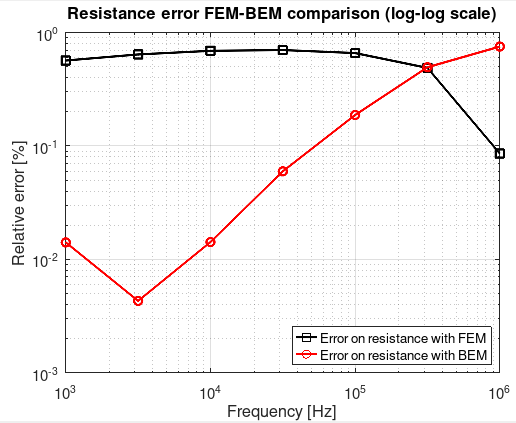
\includegraphics[width=\textwidth]{Images/bem-fem_resistance.png}
            \caption{Resistance error comparison between BEM and FEM as a function of frequency.}
        \end{figure}
    \end{minipage}\hfill
    \begin{minipage}{0.49\textwidth}
        \centering
        \begin{figure}[H]
            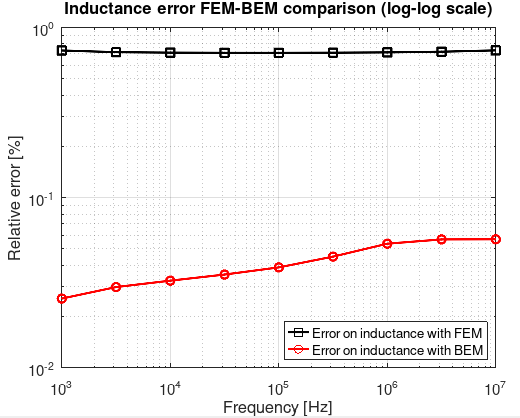
\includegraphics[width=\textwidth]{Images/bem-fem_inductance.png}
            \caption{Inductance error comparison between BEM and FEM as a function of frequency.}
        \end{figure}
    \end{minipage}
    \end{center}
\end{frame}

\section{Conclusion}
\begin{frame}{Conclusion}
    \begin{itemize}
        \item The FEM implementation for the eddy currents in two circular conductors is working correctly.
        \item The results are consistent with the analytical solution, with a relative error below 1\% for the resistance and inductance in the frequency range from $10^3$ Hz to $10^6$ Hz.
        \item The skin effect is visible in the current density distribution, with the current density decreasing exponentially with depth in the conductors.
        \item The mesh refinement is crucial for accurate results, especially at high frequencies where the skin depth is small.
        \item Future work could involve exploring different geometries and materials to further validate the FEM approach. The code can be easily adapted to other geometries and more than two conductors.
    \end{itemize}
\end{frame}

% References
\begin{frame}{References}
    \footnotesize
    \begin{thebibliography}{99}
        \bibitem{weiss1982} J. Weiss, Z. J. Csendes, ``A One-Step Finite Element Method for Multiconductor Skin Effect Problems,'' \emph{IEEE Transactions on Power Apparatus and Systems}, Vol. PAS-101, No. 10, pp. 3790-3797, October 1982.
        \bibitem{rylander2013}
        T. Rylander, A. Bondeson, P. Ingelström, \emph{Computational Electromagnetics}, Second Edition, Texts in Applied Mathematics, Vol. 51, Springer, 2013. (See Chapter 6)
        \bibitem{dirienzo_lectures}
        L. Di Rienzo, ``Lecture Notes for Computational Electromagnetics,'' Politecnico di Milano, Academic Year 2024--2025.
    \end{thebibliography}
\end{frame}


\end{document}